% Owner-review draft, 2026-10-12. No submission, acceptance, or publisher identifier.
\documentclass[journal,10pt]{IEEEtran}
\usepackage{amsmath,amssymb,graphicx,booktabs,array,url,cite}
\usepackage[hidelinks]{hyperref}
\newcommand{\ind}{\mathbf{1}}
\newcommand{\TN}{\mathrm{T}}
\newcommand{\NTN}{\mathrm{N}}
\title{Service Qualification and Shared-Power Limits in Terrestrial--Non-Terrestrial Fallback: A Reproducible Synthetic Benchmark}
\author{Edmund Gunn, Jr.\thanks{Edmund Gunn, Jr. is an independent researcher. ORCID: \href{https://orcid.org/0009-0004-6546-2609}{0009-0004-6546-2609}. Research affiliation, contact information, funding, and human verification require owner confirmation before submission. This is an unpublished owner-review draft.}}
\markboth{Owner-Review Draft, October 12, 2026}{Gunn: Service Qualification and Shared-Power Limits}
\begin{document}
\maketitle
\begin{abstract}
A backup communication path can remain connected while failing the service it is intended to preserve. This paper studies that distinction in a transparent terrestrial--non-terrestrial fallback benchmark with explicit latency, capacity, visibility, and shared-power constraints. Four deterministic selection policies are evaluated using a frozen synthetic protocol with 30 shared random seeds and 48 abstract steps per run. A mathematical characterization explains when their useful-service outcomes are identical and when preferring a nonqualifying satellite path displaces a qualifying terrestrial path. In the compound-outage base case, the terrestrial-only mean useful-service fraction is 0.7375 and the three satellite-aware policies each attain 0.8292. The paired increase is 0.09166, with a 95 percent interval of 0.07576 to 0.10756 over simulation seeds. For a configured 550 ms satellite delay exceeding a 500 ms service limit, or 0.5 Mbps satellite capacity below a 1 Mbps requirement, satellite-first service falls to 0.1083, while terrestrial-first and adaptive selection retain 0.7375. Common terminal-power loss imposes a population useful-service ceiling of 0.85 regardless of visibility. The results support a reproducible service-qualification counterexample and an audit of policy equivalence within the model. They do not establish measured satellite performance, deployed control, validated local or peer fallback, or general superiority of adaptive orchestration.
\end{abstract}
\begin{IEEEkeywords}
non-terrestrial networks, service continuity, compound outages, system resilience, reproducibility, minimum-useful service.
\end{IEEEkeywords}

\section{Introduction}
\IEEEPARstart{N}{on-terrestrial} connectivity is often proposed as a resilience layer when terrestrial access fails. The proposal is reasonable at the architectural level, but an available alternative link does not automatically deliver a useful application service. Delay, capacity, terminal power, and link visibility can each prevent service, even if a controller reports that a connection exists. A meaningful evaluation must therefore state both the fallback rule and the service qualification rule.

The established literature already addresses terrestrial--non-terrestrial integration, service continuity, and emergency use cases \cite{lin2021,rinaldi2020,azari2022}. The question here is deliberately narrower: what conclusions can be reproduced from an existing low-complexity seeded fallback engine, and which apparent policy advantages follow directly from its assumptions? An auditable benchmark is valuable when it reveals the boundary between a scientific result and an artifact of policy naming or preconfigured inputs. It should also expose unfavorable operating regions rather than report only a satellite-friendly base case.

We analyze the existing RQ3 engine in \texttt{ntn-resilience-sim}. Its frozen protocol specifies terrestrial-only, satellite-first, terrestrial-first fallback, and adaptive selection; independent Bernoulli path events; a shared power failure; latency and capacity grids; and unfavorable delay and capacity probes. The scenario identifier \texttt{gary\_emergency} denotes a synthetic configuration. It does not identify a measurement campaign, local deployment, commercial operator, or emergency-service assessment.

The contributions are threefold. First, we specify the implemented policy model mathematically and derive useful-service expectations, policy-equivalence conditions, and the shared-power ceiling. Second, we reproduce the 30-seed accepted-main experiment and report paired uncertainty, the unfavorable probes, and secondary metrics directly from its output. Third, we audit provenance and interpretation: a stale four-seed manuscript summary is separated from the later 30-seed result; capacity and visibility settings are treated as configured sensitivity parameters; and unsupported edge, peer, and field claims are excluded.

These are methodological and reproducibility contributions within a restricted model. We do not claim the first TN--NTN simulator, a new physical-layer technique, an optimal disaster controller, or a superior adaptive policy. In particular, recent lightweight disaster-simulation work \cite{wang2026} makes a broad simulator-novelty claim untenable. Establishing transferable journal-level originality will require external review and evaluation beyond this one synthetic scenario.

\section{Related Work and Positioning}
Lin et al. \cite{lin2021} explain the adaptations needed to support satellite access across radio, core, service, and terminal aspects of 5G. Their discussion of long propagation delays and quality-of-service classes motivates explicit service thresholds. It does not validate the numerical settings or stochastic failures used here. Rinaldi et al. \cite{rinaldi2020} review NTN integration and continuity issues, while Azari et al. \cite{azari2022} survey the broader progression toward integrated ground--air--space systems. Those architectural surveys establish that integration and resilience are existing research themes, rather than novel ideas introduced by this benchmark.

Capacity is architecture dependent. Sedin et al. \cite{sedin2020} evaluate NR throughput and capacity using satellite, terminal, spectrum, and geographic assumptions. Their results cannot be transferred to a single configured 5 Mbps service path without a corresponding link and resource model. We consequently use capacity as a sensitivity input, not as a measured or standards-mandated property.

Two recent studies sharpen the comparison. Wang et al. \cite{wang2026} present a lightweight post-disaster TN--NTN simulator with failure-driven migration, load-aware association, and feeder-capacity and migration penalties. Their preprint addresses the same broad simulation purpose with a richer network abstraction. Figaro et al. \cite{figaro2026} evaluate end-to-end NTN behavior using ns-3 with 3GPP calibration, including the dependence of delay and throughput on orbit, frequency, and load. These studies show why a simple Bernoulli model must not be presented as protocol-accurate or calibrated.

The specific distinction pursued here is explicit qualification of an available path against a service requirement, together with a common local-power failure that defeats both access alternatives. We provide an analytical check of the implemented engine rather than claim numerical superiority over those studies. We have not reimplemented their models or run an information-equivalent cross-simulator comparison. The bibliography audit records whether full text, abstract, or metadata was inspected; it does not infer novelty from the existence of citations.

The three-paper program also imposes a nonduplication boundary. Paper I concerns minimum-useful-service classification across workloads and device capabilities. Paper II concerns radio-aware orchestration and held-out policy comparisons. Paper III uses a fixed service threshold to isolate TN--NTN path qualification and shared failure. This paper does not reuse another paper's fixture performance as additional independent NTN validation.

\section{System Model}
\subsection{State, Inputs, and Evidence Boundary}
Let $t\in\{1,\ldots,H\}$ denote an abstract simulation step, with $H=48$. There is no specified duration in seconds. Define raw terrestrial availability $R_t$, raw NTN visibility $V_t$, and terminal-power availability $P_t$. The sampler draws three uniform random values per step, in that order, from Python's seeded pseudorandom generator and thresholds them to produce
\begin{equation}
 R_t\sim\mathrm{Bernoulli}(r),\quad V_t\sim\mathrm{Bernoulli}(v),\quad P_t\sim\mathrm{Bernoulli}(q).
\end{equation}
Here $r=1-p_R$ and $q=1-p_P$. The model assumes independence of the raw draws and independence across steps. A seed deterministically specifies the entire timeline. Comparable policies receive the same seed and parameters, and thus the same raw timeline.

In the compound condition, usable path availability is
\begin{equation}\label{eq:availability}
 A_{\TN,t}=P_tR_t,\qquad A_{\NTN,t}=P_tV_t.
\end{equation}
In the simple condition, $A_{\TN,t}=R_t$ and $A_{\NTN,t}=V_t$. Power is therefore a common disabling factor, not an additional independent radio outage. The power variable is an on/off gate; it is not a battery discharge, photovoltaic, terminal energy-consumption, or backup-generator model.

Each path $j\in\{\TN,\NTN\}$ has configured capacity $C_j$ and latency $L_j$. Values are constant during a run. There is no packet queue, fading, contention, congestion, constellation geometry, propagation calculation, or handover delay. The engine's delay is the scalar supplied to the service predicate. Although a protocol field describes the configured GEO value as RTT, the engine does not resolve one-way versus round-trip application semantics. Threshold comparisons are internally consistent scalar comparisons; application-level interpretation remains uncalibrated.

The historical registry labels several inputs as literature backed and cites 3GPP TR 38.821 \cite{tr38821}. That report provides NTN architectural and technical context. A context citation alone does not establish an exact visibility probability of 0.85, a per-service 5 Mbps capacity, or an end-to-end 40 ms latency. This paper conservatively labels these numerical inputs configured assumptions. It preserves the registry and frozen protocol rather than silently correcting their historical wording.

\subsection{Minimum-Useful Service}
The fixed qualification indicator is
\begin{equation}\label{eq:qualification}
 g_j=\ind\{C_j\ge C_{\min}\}\ind\{L_j\le L_{\max}\},
\end{equation}
with $C_{\min}=1$ Mbps and $L_{\max}=500$ ms. Equality qualifies. Let $X_{\pi,t}\in\{\TN,\NTN,\varnothing\}$ be the path selected by policy $\pi$, where $\varnothing$ is offline. Define
\begin{align}
 M_{\pi,t}&=\ind\{X_{\pi,t}\ne\varnothing\}g_{X_{\pi,t}},\\
 S_{\pi,s}&=H^{-1}\sum_{t=1}^{H}M_{\pi,t},\label{eq:service}\\
 U_{\pi,s}&=H^{-1}\sum_{t=1}^{H}\ind\{X_{\pi,t}\ne\varnothing\}.
\end{align}
$S$ is useful-service fraction, whereas $U$ is selected-path uptime. In the feasible base case they coincide. In the unfavorable probes they can diverge sharply. Neither quantity is packet delivery ratio, measured throughput, availability of a commercial service, nor success of an actual emergency workflow.

Offline selection has $M=0$ in this engine. A broader product can allow cached local or peer execution, but those paths are absent from the seeded RQ3 engine. Contract tests of another decision adapter and campus reporting fixtures do not demonstrate local or peer continuity in the experiment reported here. The benchmark therefore evaluates terrestrial, NTN, and offline outcomes only.

\subsection{Selection Rules}
The names in the source are retained for reproducibility, with descriptive labels used in figures. Terrestrial baseline selects TN if $A_\TN=1$ and otherwise goes offline. Static NTN selects NTN if $A_\NTN=1$, otherwise TN if $A_\TN=1$. It is consequently satellite first rather than an exclusive satellite-only policy. Fallback selects TN if available and otherwise NTN if available. It does not screen the backup against the service requirement before selection.

Adaptive selection forms available candidates $\mathcal A_t=\{j:A_{j,t}=1\}$ and qualifying candidates $\mathcal Q_t=\{j\in\mathcal A_t:g_j=1\}$. Its rule is
\begin{equation}
 X_{a,t}=\begin{cases}
 \varnothing,&\mathcal A_t=\emptyset,\\
 \arg\min_{j\in\mathcal B_t}(L_j,-C_j),&\text{otherwise},
 \end{cases}\quad
 \mathcal B_t=\begin{cases}\mathcal Q_t,&\mathcal Q_t\ne\emptyset,\\\mathcal A_t,&\mathcal Q_t=\emptyset.\end{cases}
\end{equation}
The pair is sorted lexicographically; identical latency and capacity retain insertion order, TN before NTN. With only two candidates, each decision has constant time and storage. It is a deterministic qualification rule, not a learning algorithm, predictive digital twin, or optimized multipath transport.

A reproducible run samples the timeline once from the seed, applies the selected rule at every step, evaluates (\ref{eq:qualification}), records path and service indicators, and aggregates (\ref{eq:service}). An unavailable path is never selected. If available paths all fail qualification, adaptive still selects an available path, giving uptime but no useful service. That behavior is essential for interpreting the unfavorable cases.

\section{Analytical Decision Boundaries}
\subsection{Expected Useful Service}
The following expectations are analytical consequences of the sampler, not additional measured results. Under (\ref{eq:availability}) and raw independence,
\begin{align}
 \mathbb E[S_b]&=qrg_\TN,\label{eq:baseline}\\
 \mathbb E[S_s]&=q\left[vg_\NTN+(1-v)rg_\TN\right],\\
 \mathbb E[S_f]&=q\left[rg_\TN+(1-r)vg_\NTN\right],\\
 \mathbb E[S_a]&=q\left[rg_\TN+vg_\NTN-rvg_\TN g_\NTN\right].\label{eq:adaptive}
\end{align}
The adaptive expression is the probability that at least one qualifying path is available. The static expression is conditioned on visibility because a visible NTN path takes priority even when it does not qualify. The fallback expression is conditioned on TN availability because TN takes priority even when it does not qualify. Thus, adaptive can differ from fallback if terrestrial service is degraded, although the frozen evaluation always configures a qualifying terrestrial path.

If $g_\TN=g_\NTN=1$, all NTN-aware policies serve precisely the same availability union for every seed and step:
\begin{equation}\label{eq:equivalence}
 M_{s,t}=M_{f,t}=M_{a,t}=P_t\ind\{R_t\lor V_t\}.
\end{equation}
Their identical service fractions do not establish adaptive superiority. They are structurally equivalent for the primary metric, even when they choose different paths. When $L_\NTN<L_\TN$, adaptive may favor NTN, while fallback favors TN; capacity and latency choices can affect usage and online delay without changing the service indicator.

\subsection{Positive, Neutral, and Harmful Regions}
For a qualifying terrestrial path, fallback and adaptive gain over baseline only when NTN also qualifies:
\begin{equation}\label{eq:gain}
 \mathbb E[S_f-S_b]=\mathbb E[S_a-S_b]=q(1-r)vg_\NTN.
\end{equation}
Their gain is positive if $q>0$, $r<1$, $v>0$, and $g_\NTN=1$. It is zero when any enabling condition fails. No negative adaptive primary-service region exists under this restricted model, because the controller can retain a qualifying available TN path and has no switching cost.

For satellite-first selection,
\begin{equation}\label{eq:staticgain}
 \mathbb E[S_s-S_b]=qv(g_\NTN-rg_\TN).
\end{equation}
If $g_\TN=1$ and $g_\NTN=0$, the difference is $-qvr$: visibility now increases harmful displacement of a usable TN path. A high-availability backup is therefore not sufficient to justify unconditional preference. Crossing the latency boundary $L_\NTN=L_{\max}$ or capacity boundary $C_\NTN=C_{\min}$ changes a binary qualification state, rather than smoothly degrading service. The current grids demonstrate that threshold behavior; they do not estimate a general delay--throughput response surface.

\subsection{Power Ceiling and Model Check}
Since $M_{\pi,t}\le P_t$, every policy satisfies
\begin{equation}\label{eq:ceiling}
 \mathbb E[S_\pi]\le q.
\end{equation}
This is a population expectation. A finite seeded realization can exceed $q$, so the figure's 0.85 line must not be interpreted as a hard bound on every sample mean. With $q=0.85$, $r=0.88$, and $v=0.85$, the analytical expectations are 0.748 for baseline, 0.8347 for feasible NTN-aware service, and 0.1122 for satellite-first service with an unqualified NTN path. The expected gain is 0.0867. These formulas provide an independent consistency check of the simulator and identify how much favorable performance is already determined by configured probabilities.

Improving visibility cannot overcome common power loss. The simple-case feasible NTN-aware expectation is $r+(1-r)v=0.982$, while compound power multiplies it by 0.85. This differs from a deployment with independently powered satellite equipment or an intact remote gateway. Such architectures require a separate prospective protocol and are not evaluated here.

\section{Experimental Design and Reproduction}
\subsection{Frozen Protocol and Provenance}
The experiment is \texttt{rq3\_gary\_failover\_sweeps}. The frozen protocol is retained at \texttt{paper/artifacts/experiment\_protocol.yaml}; the executing specification is \texttt{configs/experiments/rq3\_gary\_failover\_sweeps.yaml}. The accepted-main source audited for this draft is commit \texttt{05aaa9a}; full commit and SHA-256 hashes are recorded in the supplementary package. The 30-seed statistical-parity revision entered through commit \texttt{7afde2e}. Reproduction used unchanged simulation, policy, statistics, and configuration files.

The current protocol declares seeds 1 through 30, shared across policies; $H=48$; $p_R=0.12$; $p_P=0.15$; compound failure enabled; $C_\TN=20$ Mbps; $L_\TN=25$ ms; base $C_\NTN=5$ Mbps, $L_\NTN=40$ ms, and $v=0.85$. Delay values $\{20,40,60\}$ ms, capacities $\{1,5,20\}$ Mbps, and visibility probabilities $\{0.5,0.85,0.99\}$ define one-dimensional sweeps and two two-dimensional grids. The declared unfavorable probes use 550 ms configured GEO delay and 0.5 Mbps capacity. A power contrast removes the shared-power outage while retaining the raw random-draw schedule.

The historical manuscript describes four seeds and older numerical summaries. Those artifacts are preserved as provenance. The submission tables use the newly reproduced 30-seed full JSON, which agrees with the accepted-main statistical report. We do not treat the later expansion of a pre-existing experiment as independently verified prospective registration. The repository labels the current seed design predeclared, but a registration claim needs a dated, independently auditable protocol-before-outcome history. The present reproduction verifies computation rather than that chronology.

\subsection{Statistics and Experimental Unit}
The experimental unit is one seeded 48-step timeline, not a packet, user, terminal, or geographic site. For $n=30$ seed fractions, the mean and interval are
\begin{equation}
 \bar S_\pi=\frac1n\sum_s S_{\pi,s},\quad
 \bar S_\pi\pm t_{0.975,n-1}\frac{\hat\sigma_\pi}{\sqrt n}.
\end{equation}
Paired differences use $D_s=S_{\pi,s}-S_{b,s}$ and the same formula over $D_s$. The shared-seed design reduces unrelated timeline variation in comparisons. We retain the engine's four-decimal seed-fraction rounding; its numerical impact is bounded by $5\times10^{-5}$ per rounded fraction. Independent SciPy recomputation checks interval endpoints from those seed records.

Intervals quantify Monte Carlo variation under fixed model assumptions. They do not quantify uncertainty about an operator, disaster probability, orbital visibility, capacity, service requirements, or model misspecification. We do not pool the 1440 steps as 1440 independent real-world samples. Nor do we interpret the 27 favorable policy--parameter records as 27 independent confirmations: they arise from nine latency--visibility combinations and three service-equivalent policies. Grid intervals are descriptive and have no multiplicity correction or family-wide significance claim.

The source also reports paired standardized effect $d_z=\bar D/\hat\sigma_D$. Absolute service-fraction differences are more interpretable for the present comparison, and remain primary. If difference variance is zero, the helper returns zero rather than a mathematically meaningful standardized effect; we avoid using that convention to interpret deterministic equivalence.

\subsection{Reproduction Procedure}
A clean checkout at the recorded commit, Python 3.12.12, PyYAML, and jsonschema reproduce the engine. The audit adds pytest, SciPy, and Matplotlib for testing, independent statistics, and figures. Exact dependency versions, commands, data dictionary, and hashes accompany the manuscript. All 37 repository tests pass after the separately versioned field-kit contract fixtures are supplied; the RQ3-focused subset independently passes 17 tests. These software checks establish internal consistency, not external scientific validation.

Tables and figures are generated from the complete newly reproduced JSON by the included plotting script. No result values are typed into an image. The original experiment scripts and frozen artifacts are not modified. Analytical expressions are separately labeled and are not added to the experimental sample size.

\section{Results}
\subsection{Feasible NTN Fallback and Policy Equivalence}
\begin{table}[t]
\centering
\caption{Compound base case; 30 seed means, 48 steps each. Intervals describe simulation variability.}
\label{tab:base}
\footnotesize
\begin{tabular}{lccc}\toprule
Policy & Service & 95\% interval & NTN fraction \\ \midrule
TN only & 0.7375 & [0.7150, 0.7600] & 0.0000 \\
NTN first & 0.8292 & [0.8106, 0.8477] & 0.7208 \\
TN first & 0.8292 & [0.8106, 0.8477] & 0.0917 \\
Adaptive & 0.8292 & [0.8106, 0.8477] & 0.0917 \\
\bottomrule\end{tabular}
\end{table}

\begin{figure}[t]
\centering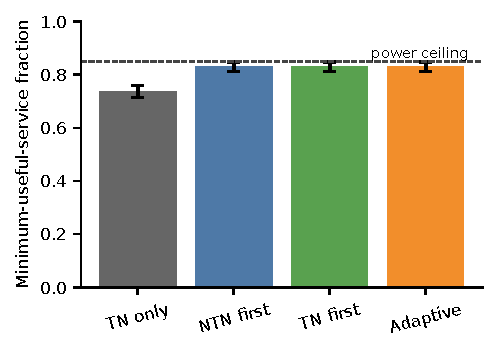
\includegraphics[width=\columnwidth]{figures/base_service.pdf}
\caption{Compound base-case service means and 95\% Student-t intervals across 30 seeds. The dashed line is the analytical population shared-power ceiling, not a realization-wise bound. All evidence is synthetic.}\label{fig:base}
\end{figure}
Table~\ref{tab:base} reports 0.7375 terrestrial-only service with interval $[0.7150,0.7600]$, versus 0.8292 and $[0.8106,0.8477]$ for each NTN-aware policy. The paired gain is 0.09166, with interval $[0.07576,0.10756]$; its seed-level standard deviation is 0.04259 and $d_z=2.1522$. Every seed exhibits a positive feasible-case gain, but this reflects an availability-union construction under favorable qualification rather than validation of a controller against a difficult competing baseline.

The three NTN-aware primary outcomes are identical for every seed, as predicted by (\ref{eq:equivalence}). Adaptive selection provides no useful-service advantage over terrestrial-first fallback. Satellite-first selection uses NTN for 0.7208 of steps, whereas fallback and adaptive use it for 0.0917. Equivalent useful service is therefore attained with very different path selection. This distinction matters before adding cost, energy, switching overhead, or billing, none of which is modeled in the seeded engine.

The observed base means are close to the analytically derived 0.748 and 0.8347. The finite-seed difference from those expectations is consistent with the reported Monte Carlo intervals. This check supports correctness of the Bernoulli mechanism, while also showing that the main favorable outcome is largely implied by its probabilities.

\begin{figure}[t]
\centering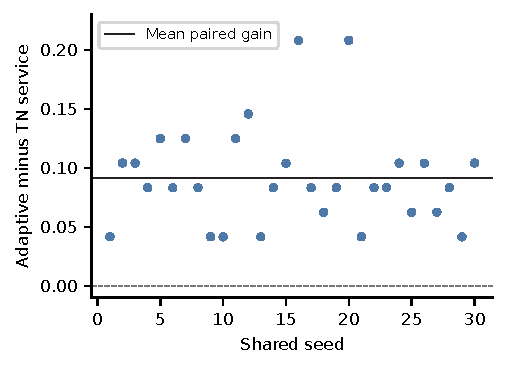
\includegraphics[width=\columnwidth]{figures/paired_seed_gain.pdf}
\caption{Paired adaptive-minus-terrestrial service gain across the 30 shared seeds in the feasible compound base case. These points are simulation runs, not subjects or measurement sessions.}\label{fig:paired}
\end{figure}

\subsection{Visibility, Capacity, and Latency Grids}
\begin{figure*}[t]
\centering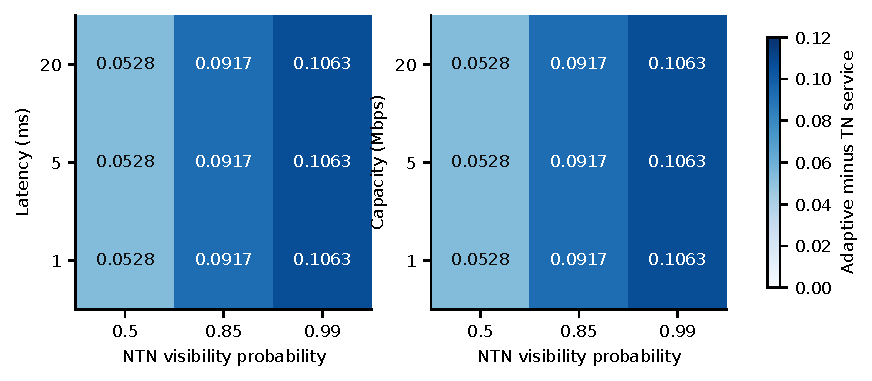
\includegraphics[width=.94\textwidth]{figures/decision_grids.pdf}
\caption{Adaptive-minus-terrestrial service fractions from the frozen grids. Capacity is held at 5 Mbps for the latency grid; delay is held at 40 ms for the capacity grid. All displayed inputs qualify under the fixed 1 Mbps/500 ms predicate. Color differences therefore follow visibility; the flat delay and capacity directions reveal model insensitivity within a qualification region.}\label{fig:grid}
\end{figure*}
The latency--visibility grid contains nine parameter combinations. All 27 NTN-aware policy--combination comparisons are favorable to baseline because each displayed latency satisfies the generous 500 ms requirement, and the configured capacity qualifies. The capacity--visibility grid similarly contains only qualifying capacities. Latency 20, 40, or 60 ms produces the same primary fraction at fixed visibility, and capacity 1, 5, or 20 Mbps does likewise. Increasing a capacity already above threshold gives no further service benefit because no throughput demand or sharing model uses it.

Figure~\ref{fig:grid} should thus be read as a discrete sensitivity audit, not a complete decision boundary map. The sampled grids omit values close to or across the 500 ms boundary and capacities below 1 Mbps, apart from the separate stress probe. The analytical threshold identifies where qualification changes, but does not validate behavior under a real orbital pass or traffic distribution. The observed favorable count alone cannot support ``NTN always improves service.''

\subsection{Unfavorable Delay and Capacity Probes}
\begin{table}[t]
\centering
\caption{Minimum-useful-service counterexamples. GEO means configured 550 ms; thin NTN means 0.5 Mbps.}
\label{tab:negative}
\footnotesize
\begin{tabular}{lccc}\toprule
Policy & LEO base & GEO & Thin NTN \\ \midrule
TN only & 0.7375 & 0.7375 & 0.7375 \\
NTN first & 0.8292 & 0.1083 & 0.1083 \\
TN first & 0.8292 & 0.7375 & 0.7375 \\
Adaptive & 0.8292 & 0.7375 & 0.7375 \\
\bottomrule\end{tabular}
\end{table}

\begin{figure}[t]
\centering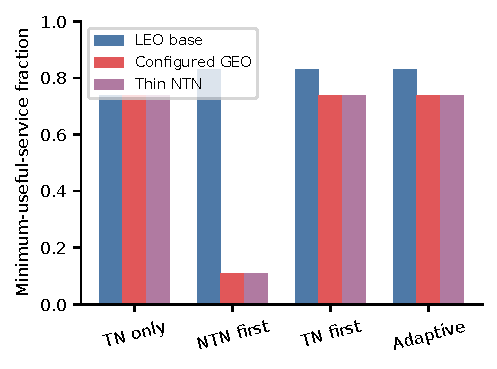
\includegraphics[width=\columnwidth]{figures/negative_cases.pdf}
\caption{Feasible LEO base case versus the two declared unqualified-NTN probes. Preferring an available but unqualified NTN path displaces terrestrial service. Terrestrial-first and adaptive retain the same primary service as baseline.}\label{fig:negative}
\end{figure}
At configured delay 550 ms, NTN fails the 500 ms qualification rule. Satellite-first useful service falls to 0.1083, while fallback and adaptive both equal the baseline's 0.7375. The 0.5 Mbps probe produces exactly the same service fractions because it sets the same binary qualification state $g_\NTN=0$ on the same visibility and outage timelines. These are distinct engineering reasons for one mathematical failure condition, not independent replications.

Satellite-first uptime remains high even though useful service collapses: it often selects a visible path that fails the predicate. Fallback can also select that path during terrestrial outages, preserving nominal online status without useful service. Adaptive screens qualifying alternatives but, when none qualify, still selects a degraded available path. This behavior demonstrates why the manuscript's primary claim uses useful service rather than uptime.

The configured GEO probe is not evidence that GEO services are generally unusable. It compares one configured scalar delay with one selected requirement. A service with a longer delay budget could qualify that same link, and real GEO designs have different resource and application characteristics \cite{figaro2026}. The negative result is a counterexample to unconditional superiority within the specified benchmark.

\subsection{Shared-Power Contrast and Secondary Metrics}
\begin{table}[t]
\centering
\caption{Power contrast on shared random streams. Simple removes the power constraint; compound disables both paths when power is lost.}
\label{tab:compound}
\footnotesize
\begin{tabular}{lccc}\toprule
Policy & Simple & Compound & Difference \\ \midrule
TN only & 0.8736 & 0.7375 & -0.1361 \\
NTN first & 0.9826 & 0.8292 & -0.1534 \\
TN first & 0.9826 & 0.8292 & -0.1534 \\
Adaptive & 0.9826 & 0.8292 & -0.1534 \\
\bottomrule\end{tabular}
\end{table}

Table~\ref{tab:compound} compares a simple radio condition with compound power loss. All policies lose useful service in the compound condition. NTN-aware policies cannot bypass the common terminal-power gate. Their additional radio availability is useful only in powered steps. The analytical ceiling (\ref{eq:ceiling}) explains the limit without attributing an observed synthetic fraction to satellite-network reliability.

\begin{table}[t]
\centering
\caption{Descriptive secondary metrics. Delay averages only selected online paths; recovery is first-miss-to-first-restoration in abstract steps.}
\label{tab:secondary}
\footnotesize
\begin{tabular}{lccc}\toprule
Policy & Delay (ms) & Offline steps & Recovery \\ \midrule
TN only & 25.00 & 12.60 & 1.60 \\
NTN first & 38.02 & 8.20 & 1.27 \\
TN first & 26.66 & 8.20 & 1.27 \\
Adaptive & 26.66 & 8.20 & 1.27 \\
\bottomrule\end{tabular}
\end{table}

For the base case, terrestrial-only average offline steps are 12.6 per run, versus 8.2 for NTN-aware policies. The first-miss recovery statistic is 1.6 abstract steps for baseline and 1.2667 for NTN-aware policies. It starts at the first service miss and stops at the first subsequent success; it does not summarize all outage spells, a disaster repair process, handover interruption, or time-to-reattach. No seconds conversion is supported.

Average online selected-path delay is 25 ms for terrestrial-only, 38.02 ms for satellite-first, and 26.66 ms for fallback and adaptive. These values are seed means of conditional path averages: offline states are excluded, and the mean is not packet weighted. They illustrate different path usage despite equal service fractions. A low conditional delay can coexist with poor service availability, so it cannot replace the primary metric.

\section{Discussion and Threats to Validity}
\subsection{What the Benchmark Establishes}
The evidence establishes reproducibility of a threshold-qualified availability model and exposes a harmful policy region that is obscured by an uptime-only report. The conjunction of an available path, adequate capacity, adequate latency, and terminal power is the central service constraint. A satellite-first rule can destroy useful service when an unqualified backup is available, whereas retaining a qualifying terrestrial path avoids that displacement.

The analytical characterization is also a guard against inflated algorithmic claims. The adaptive policy has access to configured service indicators and instantaneous path states without estimation error. Its feasible-case equivalence with simpler fallback is expected. Adding a sophisticated policy name does not create an independent contribution or additional evidence. The current synthetic results support the policy-equivalence result and unfavorable counterexample more strongly than any optimization claim.

The choice of minimum-useful service is useful for integration with a broader service-continuity program, but transfer depends on workload-specific requirements. One fixed 1 Mbps/500 ms predicate cannot represent every conversational, educational, administrative, telemetry, or emergency workload. Requirements should be independently justified before prospective application tests. A relaxed delay budget changes the GEO outcome; stricter capacity or delay requirements can eliminate the apparent LEO gain.

\subsection{Failure and Network Realism}
Independent memoryless Bernoulli events omit outage duration, spatial correlation, correlated weather, restoration processes, orbit windows, antenna obstruction, gateway failure, backhaul loss, congestion after mass failover, and common infrastructure beyond local power. These omissions can materially alter both the availability gain and the distribution of recovery time. The compound condition deliberately represents common power, but it does not model a realistic dependency graph across terminals, gateways, and core networks.

Constant capacity is particularly limiting after widespread terrestrial outage. The model gives the same configured NTN capacity regardless of the number of users seeking backup. It cannot test whether aggregate failover saturates a feeder link or whether fairness prevents each workload from meeting its requirement. Likewise, constant latency omits queueing and transport behavior. The richer models in \cite{wang2026,figaro2026} identify methodological directions for a prospective cross-check, not evidence already supplied by this engine.

A perfectly informed adaptive selector, with instantaneous switching and no penalty, cannot lose useful service relative to retaining a qualifying TN path. That built-in property is a limitation for investigating policy regret. Physical attachment, signaling, hysteresis, stale state, switch timing, packet reordering, and terminal energy would create genuine tradeoffs. None is validated here. Registry entries for handover delay or energy proxies are not evidence that those quantities participate in the reported experiment.

\subsection{Statistics, Originality, and External Validity}
Thirty reproducible seeds improve Monte Carlo characterization, but cannot resolve inaccurate assumptions. Short timelines produce coarse fractions and first-event recovery estimates. Repeated cells reuse the same random stream; latency and capacity sweeps often merely repeat a binary qualification state. We report paired uncertainty for the base comparison and descriptive contrasts elsewhere, without claiming a universal statistical result or population estimate for Gary or other named regions.

The contribution remains scientifically modest: an independently reproducible service predicate, a policy-equivalence audit, and a shared-power counterexample are transparent, but the probability derivations are elementary. Existing disaster-aware simulators undermine a broad novelty claim. No external reviewer has yet established that this focused methodological combination meets a journal's originality threshold. A larger prospective experiment should test a justified workload, correlated failures, independent backup power, and traffic-dependent NTN constraints before asserting transferable deployment value.

No RF measurement, operator attachment, deployed TN--NTN control, terminal power campaign, validated local/peer recovery, or comparison to commercial satellite service is reported. Separate host or device evidence in the wider repository program cannot be transferred into these claims. Likewise, a passing claim-firewall checker only enforces software labels; it does not certify scientific truth or independent reproduction.

\subsection{Prospective Evidence Upgrade}
A useful next study would preserve the present benchmark as an analytic control while adding a new versioned protocol. That protocol should state service requirements and units before outcomes are inspected, define gateway and terminal dependency assumptions, preregister policy information access, include capacity sharing and switch costs, and reserve independent scenarios or traces for evaluation. Field work should log terminal power, availability, end-to-end delay, delivered goodput, and application completion, with privacy and licensing review for actual traces. These are requirements for future evidence; no corresponding measurements are invented here.

\section{Conclusion}
In the reproduced synthetic model, qualifying NTN backup improves useful service over terrestrial-only access, but adaptive, terrestrial-first, and satellite-first rules have identical primary service in the favorable base case. Satellite-first selection performs poorly when a visible NTN path fails the declared delay or capacity requirement. Shared terminal-power failure constrains all policies. The mathematical boundaries explain these outcomes and prevent an uptime or policy-label advantage from being mistaken for application continuity or algorithmic superiority. The package is prepared for owner scientific review, with originality, calibration, and external-validation gaps explicitly retained.

\section*{Data and Software Availability}
Simulation source is available in \url{https://github.com/gunnchOS3k/ntn-resilience-sim} at the commit specified in the supplementary reproduction record. The repository's MIT license governs existing software and documentation. This draft's complete synthetic JSON, data dictionary, seed statistics, plotting sources, and hashes accompany the manuscript under \texttt{paper/submission/}. No field dataset is included. No permanent archive DOI, publisher DOI, or ORCID work entry has been assigned to this unpublished draft.

\section*{Acknowledgment and Declarations}
OpenAI Codex assisted substantially with literature discovery and bibliographic verification, source auditing, mathematical exposition, drafting all manuscript sections, and generation of reproducibility, statistics, and plotting scripts in this owner-review revision. Figures are deterministic plots of reproduced synthetic outputs rather than generated illustrations. The author must review and verify all calculations, citations, figures, claims, and declarations before submission; that human verification has not yet occurred. AI systems are not authors.

The proposed human author is Edmund Gunn, Jr., based on the established project attribution. Author contributions, the use of gunnchOS Research as affiliation, contact details, funding, competing interests, ownership, prior dissemination, and permission for journal submission require owner confirmation in the accompanying worksheet. No University of Oulu appointment, enrollment, supervision, institutional endorsement, or funding is claimed. The study reports synthetic software experiments and contains no human-participant or personal-network measurement data.

\bibliographystyle{IEEEtran}
\bibliography{references}
\end{document}
